\newif\ifanonymous
%\anonymoustrue%uncomment for submission version

\documentclass{llncs}

\usepackage[hmargin=3cm,vmargin=2.8cm]{geometry}

\usepackage{amsmath,amssymb}
\usepackage{ifthen}
\usepackage{subcaption}
\usepackage{booktabs}
\usepackage{siunitx}
\usepackage[section]{placeins}
\usepackage[hidelinks]{hyperref}

\usepackage{xcolor}
\definecolor{blue_link}{RGB}{0,0,200}
\hypersetup{
  colorlinks = true,
  linkcolor = blue_link,
  citecolor = blue_link,
  urlcolor = blue_link,
  bookmarksdepth = 3
}

\usepackage{tikz}
\usetikzlibrary{calc,math}

\makeatletter
\pgfdeclareshape{oplus}{%{{{
  \inheritsavedanchors[from=circle]
  \inheritanchorborder[from=circle]
  \foreach \s in {center,mid,base,text, north,south,west,east,
                  mid west,mid east,base west,base east,
                  north west,south west,north east,south east} {
    \inheritanchor[from=circle]{\s}
  }
  \backgroundpath{%
    \pgfutil@tempdima=\radius%
    \pgfmathsetlength{\pgf@xb}{\pgfkeysvalueof{/pgf/outer xsep}}%  
    \pgfmathsetlength{\pgf@yb}{\pgfkeysvalueof{/pgf/outer ysep}}%  
    \ifdim\pgf@xb<\pgf@yb%
      \advance\pgfutil@tempdima by-\pgf@yb%
    \else%
      \advance\pgfutil@tempdima by-\pgf@xb%
    \fi%
    \pgfpathcircle{\centerpoint}{\pgfutil@tempdima}%
    % north-south
    \centerpoint\advance\pgf@y by\radius  \pgf@xa=\pgf@x \pgf@ya=\pgf@y
    \centerpoint\advance\pgf@y by-\radius \pgf@xb=\pgf@x \pgf@yb=\pgf@y
    \pgfpathmoveto{\pgfpoint{\pgf@xa}{\pgf@ya}}
    \pgfpathlineto{\pgfpoint{\pgf@xb}{\pgf@yb}}
    % east-west
    \centerpoint\advance\pgf@x by\radius  \pgf@xa=\pgf@x \pgf@ya=\pgf@y
    \centerpoint\advance\pgf@x by-\radius \pgf@xb=\pgf@x \pgf@yb=\pgf@y
    \pgfpathmoveto{\pgfpoint{\pgf@xa}{\pgf@ya}}
    \pgfpathlineto{\pgfpoint{\pgf@xb}{\pgf@yb}}
  }
}%}}}
\makeatother
\tikzset{op/.style={draw, fill=none, minimum size=1.25ex, inner sep=0pt}}
\tikzset{opxor/.style={op, shape=oplus}}
\tikzset{opand/.style={op, rectangle, rounded corners=2pt, minimum height=3ex}}
\tikzset{oprot/.style={op, rectangle, rounded corners=2pt, inner sep=2pt, minimum width=3ex, font=\scriptsize}}
\tikzset{optee/.style={shape=circle, fill, draw, inner sep=0pt, minimum size=2pt}}
\tikzset{next/.style={->, >=latex}}
\tikzset{trail/.style={line width=2pt, line cap=round}}
\definecolor{delta}{HTML}{B58900}
\definecolor{epsil}{HTML}{CB4B16}
\definecolor{gamma}{HTML}{6C71C4}
\definecolor{beta}{HTML}{268BD2}
\definecolor{alpha}{HTML}{859900}

%\definecolor{mybase0}{HTML}{839496}
%\definecolor{mybase1}{HTML}{93A1A1}
%\definecolor{mybase2}{HTML}{EEE8D5}
%\definecolor{mybase3}{HTML}{FDF6E3}
%\definecolor{myred}{HTML}{DC322F}
%\definecolor{mymagenta}{HTML}{D33682}
%\definecolor{mycyan}{HTML}{2AA198}

\newcommand{\cipher}[1]{\textsf{#1}}

\newif\ifsubstates\substatesfalse

\newcommand{\printstate}{
  \ifsubstates \pgfmathsetmacro{\roundsep}{1.25}
  \else        \pgfmathsetmacro{\roundsep}{0.80} \fi
  \pgfmathsetmacro{\opoffset}{.1}

  \ifsubstates
    \foreach \r in {-2,...,4} {
      \foreach \w in {0,...,4} {
        \draw[thick] (\w-.5,-\r*\roundsep) -- ++(0,-.25);
        \node[minimum width=1*1.0cm,minimum height=.25*1.5cm, inner sep=0pt] (W\r\w) at (\w,-\r*\roundsep-.125) {};
      }
      \draw[thick] (-.5,-\r*\roundsep) node[below left, inner sep=0pt, xshift=-3pt] {$S_{\r,*}^{\r}$} rectangle ++(5,-.25);
    }
    \node[minimum width=1*1.0cm,minimum height=.25*1.5cm, inner sep=0pt] (W-1-1) at (-1,--1*\roundsep-.125) {};
    \node[minimum width=1*1.0cm,minimum height=.25*1.5cm, inner sep=0pt] (W-2-1) at (-2,--1*\roundsep-.125) {};
  \else
    \foreach \r in {-1,...,4} {
      \foreach \w in {0,...,4} {
        \coordinate (W\r\w) at (\w,-\r*\roundsep-.125);
      }
    }
    \foreach \w in {0,...,4} {
      \coordinate (W-2\w) at (\w,--2.375*\roundsep-.125);
    }
    \coordinate (W-1-1) at (-1,--1*\roundsep-.125);
    \coordinate (W-2-1) at (-2,--1*\roundsep-.125);
  \fi

  %\foreach \r/\rot in {-1/0,0/5,1/31,2/7,3/22,4/13} { % round
  \foreach \r/\rot in {-1/0,0/b_0,1/b_1,2/b_2,3/b_3,4/b_4} { % round
    \ifthenelse{\equal{\r}{-1}}{
      \pgfmathsetmacro{\txorx}{int(mod(\r+2,5))}
      \pgfmathsetmacro{\tanAx}{int(mod(\r+4,5))}
      \pgfmathsetmacro{\tanBx}{int(mod(\r+3,5))}
      \pgfmathsetmacro{\tlllx}{int(mod(\r+1,5))}
    }{
      \pgfmathsetmacro{\txorx}{int(mod(\r+3,5))}
      \pgfmathsetmacro{\tanAx}{int(mod(\r+2,5))}
      \pgfmathsetmacro{\tanBx}{int(mod(\r+1,5))}
    }
    \pgfmathsetmacro{\rprev}{int(\r-1)}
    \ifthenelse{\equal{\r}{-1}}%
    { \node[opxor] (lll\r) at ($(W\r\r) +(0,\opoffset+.25)$)  {}; }%
    { \node[oprot] (lll\r) at ($(W\r\r) +(0,\opoffset+.25)$)  {$\lll\!\rot$}; }
      \node[opxor] (xor\r) at ($(W\r\r) +(0,\opoffset+.50)$)  {};
      \node[opxor] (xnd\r) at ($(W\r\r) +(0,\opoffset+.75)$)  {};
    \ifthenelse{\equal{\r}{4}}
    { \node[opand] (and\r) at ($(W\r3) +(.5,\opoffset+.75)$)  {$\cdot$}; }
    { \node[opand] (and\r) at ($(W\r\r) +(.5,\opoffset+.75)$) {$\cdot$}; }
    \ifthenelse{\equal{\r}{-1}}%
    { \node[inner sep=1pt] (M) at ($(xnd\r) +(0,.45)$) {$M$};
      \node[inner sep=1pt] (C) at ($(lll\r) +(0,-.5)$) {$C$};
      \draw[next] (M) -- (xnd\r);
      \draw[next] (lll\r) -- (C);
      \coordinate[optee] (tlll\r) at ($(W\r\tlllx) +(0,\opoffset+.25)$); }{}
      \coordinate[optee] (txor\r) at ($(W\r\txorx) +(0,\opoffset+.50)$);
      \coordinate[optee] (tanA\r) at ($(W\r\tanAx) +(0,\opoffset+.675)$);
      \coordinate[optee] (tanB\r) at ($(W\r\tanBx) +(0,\opoffset+.825)$);

    \ifthenelse{\equal{\r}{-1}}%
    { \draw[next] (tlll\r) -- (lll\r); }{}
      \draw[next] (txor\r) -- (xor\r);
    \ifthenelse{\tanAx < \r}%
    { \draw[next] (tanA\r) -- (tanA\r-|and\r.west); }%
    { \draw[next] (tanA\r) -- (tanA\r-|and\r.east); }
    \ifthenelse{\tanBx < \r}%
    { \draw[next] (tanB\r) -- (tanB\r-|and\r.west); }%
    { \draw[next] (tanB\r) -- (tanB\r-|and\r.east); }
    \draw[next] (and\r) -- (xnd\r);
    \draw[    ] (xnd\r) -- (xor\r);
    \draw[    ] (xor\r) -- (lll\r);

    \foreach \w in {0,...,4} {
      \ifthenelse{\equal{\w}{\r}}{
        \draw (W\rprev\w) -- (xnd\r);
        \draw (lll\r) -- (W\r\w);
      }{
        \draw (W\rprev\w) -- (W\r\w);
      }
    }
  }
}

%new commands
\newcommand{\bias}{\ensuremath{\operatorname{bias}}}
\newcommand{\weight}{\ensuremath{\operatorname{weight}}}
\newcommand\eqdef{:=}%equality by definition
\newcommand\StateUpdate{\ensuremath{\texttt{StateUpdate}}}
\newcommand\rotl{\ensuremath{\lll}}
\newcommand\rotlxy{\ensuremath{\lll_W}}

\ifanonymous
\author{}
\institute{}
\else
\author{Tomer Ashur, Maria Eichlseder, Ga\"etan Leurent,\\Brice Minaud, Yann Rotella, Beno\^it Viguier, Yu Sasaki}
\institute{}
%\path|tomer.ashur@esat.kuleuven.be|, \path|maria.eichlseder@iaik.tugraz.at|, \path|gaetan.leurent@inria.fr|, \path|brice.minaud@gmail.com|, \path|yann.rotella@inria.fr|, \path|b.viguier@science.ru.nl|, \path|sasaki.yu@lab.ntt.co.jp|
\fi

\begin{document}

\mainmatter

\title{Note on Linear Biases in MORUS}

\maketitle

\begin{abstract}
In this note, we show the existence of linear biases in the output of the authenticated encryption scheme MORUS. More precisely, we show that when encrypting a fixed plaintext multiple times, a linear correlation exists between some bits at the output of the cipher. Moreover the bias depends purely on the plaintext, and not on the secret key of the cipher. In principle, this property could be used to recover unknown bits of a plaintext encrypted a large number of times, provided an initial segment of the plaintext is fixed and known. However, the biases are quite small: for the smaller MORUS640 variant, claiming a security level of 128 bits, the bias is $2^{-73}$, and would thus require around $2^{146}$ encryptions to be exploited directly; for MORUS1280, claiming a security level of 256 bits, the bias is $2^{-76}$, corresponding to a data requirement of $2^{152}$ encryptions. We note that rekeying does not prevent the attack: the biases are independent of the secret encryption key, and can be exploited as long as a given plaintext is encrypted enough times, regardless of whether each encryption uses a different key.
\keywords{Linear Cryptanalysis, MORUS, CAESAR.}
\end{abstract}

\section{Introduction}

Our main result is the existence of a linear trail linking ciphertext bits spanning five consecutive encryption steps. As a consequence of this trail, we exhibit a biased linear combination of ciphertext bits, which holds across any given sequence of five consecutive encryption steps. Technically, this assumes that the inner state of the cipher at the start of the trail is uniformly random, but this is a fair assumption since the inner state should be indistinguishable from uniform randomness by design. Moreover, that is the only assumption required; in particular, the secret key or the nonce used to initalize the inner state of MORUS are irrelevant: the bias will exist regardless of their value.

\section{Notation}

We define the \emph{bias} of an event $E$ as:
\[
\bias(E) \eqdef 2\Pr(E)-1.
\]
Note that the bias is sometimes defined as half the above value in the literature. We also define the \emph{weight} of an event as:
\[
\weight(E) \eqdef -\log|\bias(E)|
\]
where $\log$ denotes logarithm in base 2. By the piling-up lemma, the bias (resp. weight) of an XOR of independent variables is equal to the product (resp. sum) of their individual biases (resp. weights).

We will also use the following notation, where an \emph{encryption step} refers to one call to the \StateUpdate{} function:\\
\centerline{
\def\arraystretch{1.25}
\begin{tabular}{lcl}
$C^t$ &:& the ciphertext block output during the $t$-th encryption step.\\
$C^t_j$ &:& the $j$-th bit of $C^t$, with $C^t_0$ being the rightmost bit.\\
$S^t_i$ &:& the $i$-th register at the beginning of $t$-th encryption step.\\
$S^t_{i,j}$ &:& the $j$-th bit of $S^t_i$, with $S^t_{i,0}$ being the rightmost bit.
\end{tabular}
}
In the remainder, the $0$-th encryption step will denote the encryption step where our linear trail starts. Any encryption step could be chosen for that purpose, as long as at least four more encryption steps follow. In particular the $0$-th encryption step from the perspective of the trail does not have to be the first encryption step after initialization.

Finally, let $x$ denote a register. Recall that register of \cipher{MORUS} are composed of four words. We now define register-wise and word-wise rotations (denoted by \texttt{<<<} and \texttt{Rotl\_xxx\_yy} respectively in the \cipher{MORUS} design document):\\
\centerline{
\def\arraystretch{1.25}
\begin{tabular}{lcl}
$x \rotl y$ &:& circular shift of $x$ by $y$ bits to the left.\\
$x \rotlxy y$ &:& circular shift of each word within $x$ by $y$ bits to the left.\\
\end{tabular}
}

\section{A Linear Bias in \cipher{MORUS}}

To simplify the description of the attack, we assume all plaintext blocks are zero. However the same results would hold as long as the plaintext is fixed. Let $w$ denote the word size, i.e. 32 for \cipher{MORUS640}, and 64 for \cipher{MORUS1280}. Recall that the inner state of the cipher consists of five $4w$-bit registers $S_0,\dots,S_4$, each containing four $w$-bit words.

\subsection{Symmetric Linear Combinations}

We begin with a few observations about the \StateUpdate{} function. Beside XOR and AND operations, the \StateUpdate{} function uses two types of bit rotations:
\begin{enumerate}
\item \emph{word-wise} rotations perform a circular shift on each word within a register;
\item \emph{register-wise} rotations perform a circular shift on a whole register.
\end{enumerate}
The second type of rotation always shifts registers by a multiple of the word size (i.e. 32 for \cipher{MORUS640}). This amounts to a (circular) permutation of the words within the register: for example, if a register contains the words $(A, B, C, D)$, and a register-wise rotation by 32 bits to the left is performed, then the register now contains the words $(B, C, D, A)$.

Since we want to build a linear trail, we are interested in linear combinations of bits within a register.
\begin{definition}
Let $w$ denote the word size in bits, and $r = 4w$ denote the register size. A linear combination of the form:
\[
S^t_{i,j(0)} \oplus S^t_{i,j(1)} \oplus \dots \oplus S^t_{i,j(k)}
\]
is said to be \emph{symmetric} iff the set of bits $S^t_{i,j(0)}, \dots, S^t_{i,j(k)}$ is left invariant by a circular shift by $w$ bits; that is, iff:
\[
\{j(i) : i\leq k\} = \{j(i) + w \text{\rm{} mod } r : i\leq k\}.
\]
\end{definition}
\emph{Example.} The following linear combination is symmetric for \cipher{MORUS640}, i.e. $w = 32$:
\begin{equation}
S^t_{0,0} \oplus S^t_{0,32} \oplus S^t_{0,64} \oplus S^t_{0,96}.
\label{eq:symmetric}
\end{equation}

This definition naturally extends to a linear combination across multiple registers, and also across ciphertext blocks.
The value of such a linear combination is unaffected by register-wise rotations, since those rotations always shift registers by a multiple of the word size.
On the other hand, since word-wise rotations always shift all four words within a register by the same amount, word-wise rotations preserve the symmetric property. Moreover, the XOR of two symmetric linear combinations is also symmetric; and the same holds for the AND operation (if we extend the symmetric property to non-linear combinations in the natural way).

This naturally leads to the idea of building a linear trail using only symmetric linear combinations, which is what we are going to do. As a result, the effect of register-wise rotations can be ignored. Moreover, since all linear combinations we consider are going to be symmetric, they can be described by truncating the linear combination to the first word of a register. Indeed, an equivalent way of saying a linear combination is symmetric, is that it involves the same bits in each word within a register. For example, in the case of (\ref{eq:symmetric}) above, the four bits involved are the first bit of each of the four words.

\subsection{\cipher{MiniMORUS}}

In fact, we can go further an consider a reduced version of \cipher{MORUS} where each register contains a single word instead of four. The \StateUpdate{} function is unchanged, except for the fact that register-wise rotations are removed: see Figure~\ref{fig:minimorus}. We call these reduced versions \cipher{MiniMORUS640} and \cipher{MiniMORUS1280}, for \cipher{MORUS640} and \cipher{MORUS1280} respectively. Since registers in \cipher{MiniMORUS} contain a single word, word-wise and register-wise rotations are the same operation; for simplicity we write $\lll$ for word-wise rotations.

Because the trail we are going to build is relatively complex, we will first describe it on \cipher{MiniMORUS640}. We will then extend it to the full \cipher{MORUS640} via the previous symmetry. The trail for \cipher{MORUS1280} will be essentially the same.

\begin{figure}[h]
  \substatesfalse
  % \substatesfalse to label state words and/or masks
  \centering
  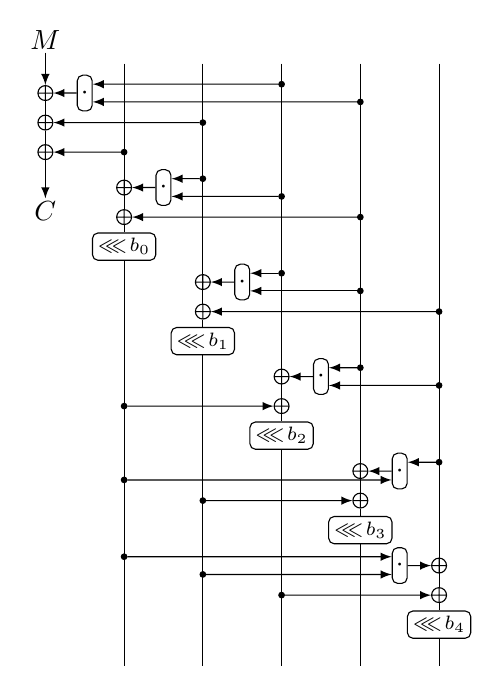
\begin{tikzpicture}[xscale=1.0,yscale=1.5]%{{{
    \printstate
  \end{tikzpicture}%}}}
  \caption{\cipher{MiniMORUS} state update function.}
  \label{fig:minimorus}
\end{figure}


\section{Linear Trail for \cipher{MiniMORUS640}}

\subsection{Overview of the Trail}

To build a linear trail on \cipher{MiniMORUS}, we combine the following five trail fragments $\alpha^t_i$, $\beta^t_i$, $\gamma^t_i$, $\delta^t_i$, $\varepsilon^t_i$, where the subscript $i$ denotes a bit position, and the superscript $t$ denotes a step number:
\begin{itemize}
    \item $\alpha^t_i$ approximates (one bit of) state word $S_0$ using the ciphertext;
    \item $\beta^t_i$ approximates $S_1$ using $S_0$ and the ciphertext;
    \item $\gamma^t_i$ approximates $S_4$ using two approximations of $S_1$ in consecutive steps;
    \item $\delta^t_i$ approximates $S_2$ using two approximations of $S_4$ in consecutive steps;
    \item $\varepsilon^t_i$ approximates $S_0$ using two approximations of $S_2$ in consecutive steps.
\end{itemize}

The trail fragments are depicted on \autoref{fig:minimorusfragments}, and may be represented as follows (recall that the $b_i$'s are rotation constants):
\begin{alignat*}{2}
\alpha^t_i:\quad&& C^t_i &\to S^{t+1}_{0,i+b_0} \\
\beta^t_i:\quad&& C^t_i, S^t_{0,i} &\to S^t_{1,i} \\
\gamma^t_i:\quad&& S^t_{1,i}, S^{t+1}_{1,i+b_1} &\to S^t_{4,i} \\
\delta^t_i:\quad&& S^t_{4,i}, S^{t+1}_{4,i+b_4} &\to S^{t+1}_{2,i} \\
\varepsilon^t_i:\quad&& S^t_{2,i}, S^{t+1}_{2,i+b_2} &\to S^{t+1}_{0,i}.
\end{alignat*}

In all cases except $\alpha^t_i$, the trail fragment approximates a single AND gate by zero, which holds with probability 3/4, and hence the trail fragment has weight 1. In the case of $\alpha^t_i$, two AND gates are involved; however the two gates share an entry in common, so their sum can be written as:
\[
x \cdot y \oplus x \cdot z = x \cdot (y \oplus z).
\]
As a result, the trail fragment $\alpha^t_i$ also has a weight of 1. Another way to look at this phenomenon is that the trail holds for two different approximations of the AND gates: the alternative approximation is depicted by a dashed line on \autoref{fig:minimorusfragments}.

\begin{figure}
  \substatesfalse
  % \substatesfalse to label state words and/or masks
  \centering
  \begin{subfigure}{.32\textwidth}
  \centering
  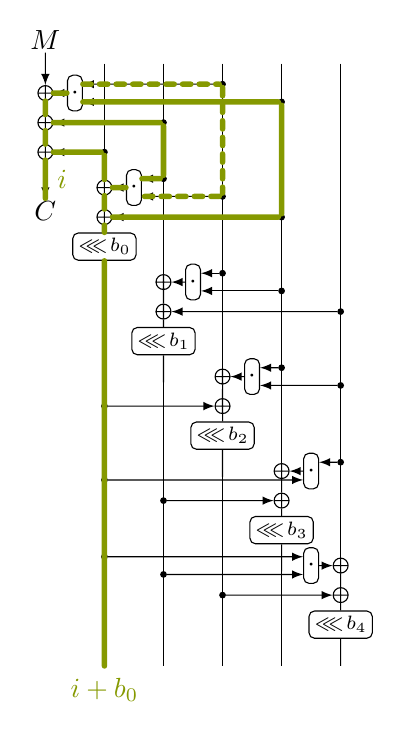
\begin{tikzpicture}[xscale=0.75,yscale=1.5]%{{{
    \printstate
    \draw[trail, alpha]
      (C) -- node[right] {$i$} (lll-1)
      (lll-1) -- (tlll-1) (lll-1) -- (xor-1) (xor-1) -- (xnd-1)
      (xnd-1) -- (and-1) (xor-1) -- (txor-1) (txor-1) -- (tanB0) (tanB0) -- (tanB0-|and0.east)
      (and0) -- (xnd0) (xnd0) -- (tlll-1) (xnd0) -- (xor0)
      (and-1.east|-tanA-1) -- (tanA-1) (tanA-1) -- (txor0) (txor0) -- (xor0)
      (xor0) -- (lll0) (lll0) -- (W40) node[below] {$i+b_0$}
      ;
    \draw[trail, alpha, dashed]
      (and-1.east|-tanB-1) -- (tanB-1) (tanB-1) -- (tanA0) (tanA0) -- (tanA0-|and0.east)
      ;
  \end{tikzpicture}%}}}
  \caption*{$\alpha_i$: weight 1 (not 2)} %$C^j_i, S^{j-1,0}_{i+5}$ ($w\!=\!1$)}
  \end{subfigure}
  \hfill
  \begin{subfigure}{.32\textwidth}
  \centering
  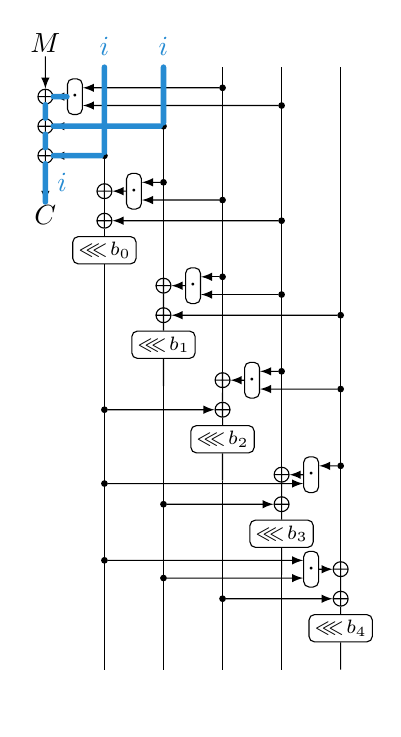
\begin{tikzpicture}[xscale=0.75,yscale=1.5]%{{{
    \printstate
    \draw[trail, beta]
      (C) -- node[right] {$i$} (lll-1)
      (lll-1) -- (tlll-1) (lll-1) -- (xor-1) (xor-1) -- (xnd-1)
      (tlll-1) -- (W-20) node[above] {$i$}
      (xor-1) -- (txor-1) (txor-1) -- (W-21) node[above] {$i$}
      (xnd-1) -- (and-1)
      (W40) node[below] {\phantom{$i$}}
      ;
  \end{tikzpicture}%}}}
  \caption*{$\beta_i$: weight 1} %$C^j_i, S^{j,0}_i, S^{j,1}_i$ ($w\!=\!0$)}
  \end{subfigure}
  \hfill
  \begin{subfigure}{.32\textwidth}
  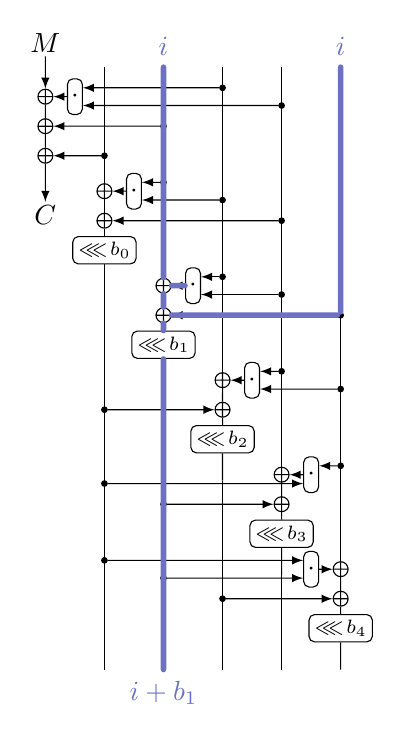
\begin{tikzpicture}[xscale=0.75,yscale=1.5]%{{{
    \printstate
    \draw[trail, gamma]
      (W-21) node[above] {$i$} -- (xnd1) (xnd1) -- (xor1) (xor1) -- (lll1)
      (xnd1) -- (and1)
      (xor1) -- (txor1)
      (txor1) -- (W-24) node[above] {$i$}
      (lll1) -- (W41) node[below] {$i+b_1$}
      ;
  \end{tikzpicture}%}}}
  \caption*{$\gamma_i$: weight 1} %$S^{j,1}_i, S^{j,4}_i, S^{j+1,1}_{i-1}$ ($w\!=\!1$)}
  \end{subfigure}
  \bigskip

  \begin{subfigure}{.32\textwidth}
  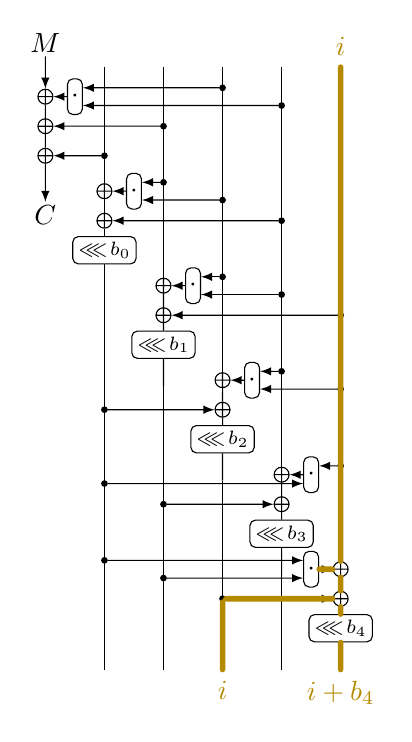
\begin{tikzpicture}[xscale=0.75,yscale=1.5]%{{{
    \printstate
    \draw[trail, delta]
      (W-24) node[above] {$i$} -- (xnd4) (xnd4) -- (xor4) (xnd4) -- (and4)
      (xor4) -- (lll4) (xor4) -- (txor4) (txor4) -- (W42) node[below] {$i$}
      (lll4) -- (W44) node[below] {$i+b_4$}
      ;
  \end{tikzpicture}%}}}
  \caption*{$\delta_i$: weight 1} %$S^{j,4_i}, S^{j+1,2}_i, S^{j+1,4}_{i+13}$ ($w\!=\!1$)}
  \end{subfigure}
  \hfill
  \begin{subfigure}{.32\textwidth}
  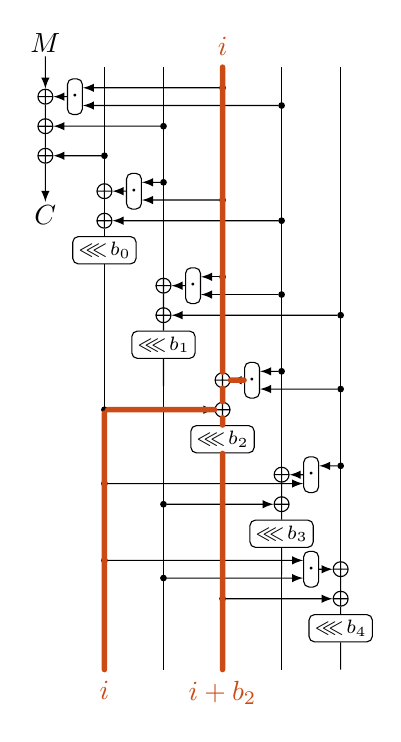
\begin{tikzpicture}[xscale=0.75,yscale=1.5]%{{{
    \printstate
    \draw[trail, epsil]
      (W-22) node[above] {$i$} -- (xnd2) (xnd2) -- (xor2) (xnd2) -- (and2)
      (xor2) -- (lll2) (xor2) -- (txor2) (txor2) -- (W40) node[below] {$i$}
      (lll2) -- (W42) node[below] {$i+b_2$}
      ;
  \end{tikzpicture}%}}}
  \caption*{$\varepsilon_i$: weight 1} %$S^{j,2}_i, S^{j+1,0}_i, S^{j+1,2}_{i+7}$ ($w\!=\!1$)}
  \end{subfigure}
  \hfill
  \begin{subfigure}{.32\textwidth}
    \small
    \begin{align*}
      \intertext{\cipher{MiniMORUS-640}:}
\alpha^t_i:&& C^t_i &\to S^{t+1}_{0,i+5} \\
\beta^t_i:&& C^t_i, S^t_{0,i} &\to S^t_{1,i} \\
\gamma^t_i:&& S^t_{1,i}, S^{t+1}_{1,i+31} &\to S^t_{4,i} \\
\delta^t_i:&& S^t_{4,i}, S^{t+1}_{4,i+13} &\to S^{t+1}_{2,i} \\
\varepsilon^t_i:&& S^t_{2,i}, S^{t+1}_{2,i+7} &\to S^{t+1}_{0,i}.
      \intertext{\cipher{MiniMORUS-1280}:}
\alpha^t_i:&& C^t_i &\to S^{t+1}_{0,i+13} \\
\beta^t_i:&& C^t_i, S^t_{0,i} &\to S^t_{1,i} \\
\gamma^t_i:&& S^t_{1,i}, S^{t+1}_{1,i+46} &\to S^t_{4,i} \\
\delta^t_i:&& S^t_{4,i}, S^{t+1}_{4,i+4} &\to S^{t+1}_{2,i} \\
\varepsilon^t_i:&& S^t_{2,i}, S^{t+1}_{2,i+38} &\to S^{t+1}_{0,i}.
    \end{align*}
    \caption*{\cipher{MiniMORUS} instances}
  \end{subfigure}
  \caption{\cipher{MiniMORUS} linear approximation fragments.}
  \label{fig:minimorusfragments}
\end{figure}

Overall, the idea is that by using $\alpha^t_i$, we are able to approximate a bit of $S_0$ using only a ciphertext bit. By combining $\alpha^t_i$ with $\beta^t_i$, we are then able to approximate a bit of $S_1$ using only ciphertext bits (from two consecutive rounds). Likewise, $\gamma^t_i$ allows us to ``jump'' from $S_1$ to $S_4$, i.e. by combining $\alpha^t_i$ with $\beta^t_i$ and $\gamma^t_i$, we are able to approximate one bit of $S_4$ using only ciphertext bits. Notice however that $\gamma^t_i$ requires approximating $S_1$ in two consecutive rounds; and so the previous combination requires using $\alpha^t_i$ and $\beta^t_i$ \emph{twice}. In the same way, $\delta^t_i$ allows us to jump from $S_4$ to $S_2$; and $\varepsilon^t_i$ allows jumping from $S_2$ back to $S_0$. In the end, we are able to approximate a bit of $S_0$ using only ciphertext bits via the combination of all trail fragments $\alpha^t_i$, $\beta^t_i$, $\gamma^t_i$, $\delta^t_i$, and $\varepsilon^t_i$.

However, the same bit of $S_0$ can also be approximated much more simply by using $\alpha^t_i$ at the corresponding step. Thus that bit can be approximated from two different sides: the first one uses a combination of all trail fragments, and involves successive approximations of all state registers (except $S_3$) spanning several encryption steps. The second only involves using $\alpha^t_i$ at the final step reached by the previous trail. By XORing up these two approximations, we are left with only ciphertext bits, spanning five consecutive encryption rounds.

Of course, the overall trail resulting from all of the previous combinations is quite complex, especially since $\gamma^t_i$, $\delta^t_i$, and $\varepsilon^t_i$ each require two copies of the preceding trail fragment in consecutive rounds: that is, $\varepsilon^t_i$ requires two approximations of $S_2$, which requires using $\delta^t_i$ twice; and $\delta^t_i$ in turn requires using $\gamma^t_i$ twice, which itself requires using $\alpha^t_i$ and $\beta^t_i$ twice. Then $\alpha^t_i$ is used one final time to close the trail. One may naturally wonder if some components of this trail are in conflict. In particular, products of bits from registers $S_2$ and $S_3$ are approximated multiple times, by $\alpha^t_i$, $\beta^t_i$ and $\gamma^t_i$. To address this concern, and ensure that all approximations along the trail are in fact compatible, we now compute the full trail equation explicitely.

\subsection{Trail Equation}

The equation corresponding to each of the five trail fragments $\alpha^t_i$, $\beta^t_i$, $\gamma^t_i$, $\delta^t_i$, $\varepsilon^t_i$ may be written explicitely as $A^t_i$, $B^t_i$, $C^t_i$, $D^t_i$, $E^t_i$ as follows. For each equation, we write on the left-hand side of the equality the biased linear combination used in the trail; and on the right-hand side, the remainder of the equation, which must have non-zero bias (in all cases the bias is $2^{-1}$).
\begin{alignat*}{2}
A^t_i:\quad&& C^t_i \oplus S^{t+1}_{0,i+b_0} &= S^t_{1,i} \oplus S^t_{3,i} \oplus S^t_{1,i} \cdot S^t_{2,i} \oplus S^t_{2,i} \cdot S^t_{3,i}\\
B^t_i:\quad&& C^t_i \oplus S^t_{0,i} \oplus S^t_{1,i} &= S^t_{2,i} \cdot S^t_{3,i} \\
C^t_i:\quad&& S^t_{1,i} \oplus S^{t+1}_{1,i+b_1} \oplus S^t_{4,i} &= S^t_{2,i} \cdot S^t_{3,i}\\
D^t_i:\quad&& S^t_{4,i} \oplus S^{t+1}_{4,i+b_4} \oplus S^{t+1}_{2,i} &= S^t_{0,i} \cdot S^t_{1,i}\\
E^t_i:\quad&& S^t_{2,i} \oplus S^{t+1}_{2,i+b_2} \oplus S^{t+1}_{0,i} &= S^t_{3,i} \cdot S^t_{4,i}
\end{alignat*}

From an algebraic point of view, building the full trail amounts to adding up copies of the previous equations for various choices of $t$ and $i$, so that eventually all $S^x_{y,z}$ on the left-hand side cancel out. Then we are left with only ciphertext terms on the left-hand side, while the right-hand side consists of a sum of biased expressions. By measuring the bias of the right-hand side expression, we will then be able to deduce the same bias on the linear combination of ciphertext bits on the left-hand side. We now set out to do so, and compute the equation of the full trail explicitely.

In order to build the equation for the full trail, we start with $E^3_0$:
\[
S^3_{2,0} \oplus S^{4}_{2,b_0} \oplus S^{4}_{0,0} = S^3_{3,0} \cdot S^t_{4,0}.
\]
In order to cancel the $S^{4}_{0,0}$ term on the left-hand side, we add in the equation $A^3_{-b_0}$ (where the sum of two equations of the form $a = b$ and $c = d$ is defined to be $a+c = b+d$). This yields:
\begin{align*}
&S^3_{2,0} \oplus S^{4}_{2,7} \oplus C^{3}_{0,-b_0}\\
=\; &S^3_{3,0} \cdot S^t_{4,0} \oplus S^t_{1,-b_0} \oplus S^t_{3,-b_0} \oplus S^3_{1,-b_0} \cdot S^3_{2,-b_0} \oplus S^3_{2,-b_0} \cdot S^t_{3,-b_0}.
\end{align*}
We then need to cancel two terms of the form $S^t_{2,i}$. To do this, we add in the equations $D^t_i$ for appropriate choices of $t$ and $i$. This replaces the two $S^t_{2,i}$ terms by four $S^t_{4,i}$ terms. By using equation $B^t_i$ four times, we can then replace these four $S^t_{4,i}$ terms by eight $S^t_{1,i}$ terms. By applying equation $B^t_i$ eight times, these eight $S^t_{1,i}$ terms can in turn be replaced by eight $S^t_{0,i}$ terms (and some ciphertext terms). Finally, applying $A^t_i$ eight times allows us to replace these eight $S^t_{0,i}$ terms by only ciphertext bits. We do not write the whole process as it is rather tedious. Ultimately, for \cipher{MORUS640}, this yields the equation:

\allowdisplaybreaks
\begin{flalign*}
&&&C^0_{27} \oplus C^1_{0} \oplus C^1_{2} \oplus C^1_{8} \oplus C^1_{26} \oplus C^2_{1} \oplus C^2_{13} \oplus C^2_{15}&&\\
&&\oplus\; &C^2_{27} \oplus C^2_{31} \oplus C^3_{6} \oplus C^3_{12} \oplus C^3_{14} \oplus C^3_{20} \oplus C^4_{19}&&\\
&&=\; &S^0_{1,27} \oplus S^0_{3,27} \oplus S^0_{1,27} \cdot S^0_{2,27} \oplus S^0_{2,27} \cdot S^0_{3,27}&&\text{weight 1}\\
&&\oplus\; &S^1_{1,26} \oplus S^1_{3,26} \oplus S^1_{1,26} \cdot S^1_{2,26} \oplus S^1_{2,26} \cdot S^1_{3,26}&&\text{weight 1}\\
&&\oplus\; &S^1_{1,8} \oplus S^1_{3,8} \oplus S^1_{1,8} \cdot S^1_{2,8} \oplus S^1_{2,8} \cdot S^1_{3,8}&&\text{weight 1}\\
&&\oplus\; &S^2_{3,1} \oplus S^2_{1,1} \oplus S^2_{1,1} \cdot S^2_{2,1} \oplus S^2_{2,1} \cdot S^2_{3,1}&&\text{weight 1}\\
&&\oplus\; &S^2_{1,7} \oplus S^2_{3,7} \oplus S^2_{1,7} \cdot S^2_{2,7} \oplus S^2_{2,7} \cdot S^2_{3,7}&&\text{weight 1}\\
&&\oplus\; &S^2_{1,15} \oplus S^2_{3,15} \oplus S^2_{1,15} \cdot S^2_{2,15} \oplus S^2_{2,15} \cdot S^2_{3,15}&&\text{weight 1}\\
&&\oplus\; &S^2_{1,27} \oplus S^2_{3,27} \oplus S^2_{1,27} \cdot S^2_{2,27} \oplus S^2_{2,27} \cdot S^2_{3,27}&&\text{weight 1}\\
&&\oplus\; &S^1_{1,2} \oplus S^1_{3,2} \oplus S^1_{1,2} \cdot S^1_{2,2} \oplus S^1_{2,2} \cdot S^1_{3,2}&&\text{weight 1}\\
&&\oplus\; &S^3_{3,14} \oplus S^3_{1,14} \oplus S^3_{1,14} \cdot S^3_{2,14} \oplus S^3_{2,14} \cdot S^3_{3,14}&&\text{weight 1}\\
&&\oplus\; &S^2_{0,0} \cdot S^2_{1,0}&&\text{weight 1}\\
&&\oplus\; &S^2_{2,31} \cdot S^2_{3,31}&&\text{weight 1}\\
&&\oplus\; &S^2_{3,0} \cdot S^2_{4,0}&&\text{weight 1}\\
&&\oplus\; &S^3_{0,7} \cdot S^3_{1,7}&&\text{weight 1}\\
&&\oplus\; &S^3_{2,6} \cdot S^3_{3,6}&&\text{weight 1}\\
&&\oplus\; &S^3_{2,12} \cdot S^3_{3,12}&&\text{weight 1}\\
&&\oplus\; &S^4_{2,19} \cdot S^4_{3,19}.&&\text{weight 1}
\end{flalign*}

\subsection{Bias of the Trail}

In the equation from the previous section, each line on the right-hand side of the equality involves distinct terms, and each line has a weight of 1. By the piling-up lemma, it follows that if we assume distinct $S^t_{i,j}$ terms to be uniform and independent, then the expression on the right-hand side has a weight of 16. Hence the linear combination of ciphertext bits on the left-hand side has a bias of $2^{-16}$.

That the bias is so high may be suprising: indeed, the full trail uses trail fragment $\varepsilon^t_i$ 1 time, $\delta^t_i$ 2 times, $\gamma^t_i$ 4 times, $\beta^t_i$ 8 times, and $\alpha^t_i$ 9 times. Since each trail fragment has a weight of 1, this would suggest that the total bias should be $1+2+4+8+9 = 24$ rather than 16. However, when combining trail fragments $\beta_i$ and $\gamma_i$, notice that the same AND is computed at the same round between registers $S_2$ and $S_3$. In both cases it is approximated by zero. When XORing the corresponding equations, these two ANDs cancel each other, which saves two AND gates. Since $\gamma^t_i$ is used four times in the course of the full trail, this results in saving 8 AND gates overall, which explains why the final bias is $2^{-16}$ rather than $2^{-24}$.

\subsection{Experiments}

To confirm that our analysis is correct, we ran experiments on an implementation of \cipher{MiniMORUS640} and \cipher{MiniMORUS1280}. In both cases, we measured the bias of two halves $\chi_1$ and $\chi_2$ of the full trail, as well as the bias of the full trail itself (denoted by $\chi$). Results are displayed on \autoref{tab:miniapproximations}. 
While our analysis from the previous section predicts a bias of $2^{-16}$, experiments confirm a slightly higher bias of $2^{-15.5}$ for \cipher{MORUS640}. The discrepancy of $2^{-0.5}$ probably arises from the fact that register bits across different rounds are not completely independent.

%\noindent
%2 approximations for $S^{2,2}_{0}$ of \cipher{MiniMORUS-640}:
%\begin{align*}
%  S^{2,2}_0 &= C^0_{27} \oplus C^1_{0, 8, 26} \oplus C^2_{7,13,31} \oplus C^3_{12} \tag{corr. $2^{-7}$} \\
%  S^{2,2}_0 &= C^1_{2} \oplus C^2_{1,7,15,27} \oplus C^3_{6,14,20} \oplus C^4_{19} \tag{corr. $2^{-9}$} \\
%\intertext{Combined ciphertext-only approximation:}
%  0 &= C^0_{27} \oplus C^1_{0, 2, 26, 8} \oplus C^2_{1,13,15,27,31} \oplus
%  C^3_{6,12,14,20} \oplus C^4_{19} \tag{corr. $\approx 2^{-15.5}$}
%\end{align*}
%\bigskip
%
%\noindent
%2 approximations for $S^{2,2}_{0}$ of \cipher{MiniMORUS-1280}:
%\begin{align*}
%  S^{2,2}_0 &= C^0_{51} \oplus C^1_{0, 33, 55} \oplus C^2_{4,37,46} \oplus C^3_{50} \tag{corr. $2^{-7}$} \\
%  S^{2,2}_0 &= C^1_{25} \oplus C^2_{7,29,38,51} \oplus C^3_{11,20,42} \oplus C^4_{24} \tag{corr. $2^{-9}$} \\
%\intertext{Combined ciphertext-only approximation:}
%  0 &= C^0_{51} \oplus C^1_{0, 25, 33, 55} \oplus C^2_{4,7,29,37,38,46,51} \oplus C^3_{11,20,42,50} \oplus C^4_{24} \tag{corr. $\approx 2^{-??}$}
%\end{align*}

\begin{table}[h!]
  \caption{Experimental verification of trail biases.}
  \label{tab:miniapproximations}
  \centerline{
  \begin{tabular}{@{}llSSS@{}}
    \toprule
    & & \multicolumn{3}{@{}c@{}}{Weight} \\
    \cmidrule{3-5}
    \multicolumn{2}{@{}l}{Approximations for \cipher{MiniMORUS640}}
             & {Exp.} & {Bool.} & {Meas.} \\
    \midrule
    $\chi_1$ & $S^{2,2}_0 = C^0_{27} \oplus C^1_{0, 8, 26} \oplus C^2_{7,13,31} \oplus C^3_{12}$
             & 7    & 7     & 7 \\
    $\chi_2$ & $S^{2,2}_0 = C^1_{2} \oplus C^2_{1,7,15,27} \oplus C^3_{6,14,20} \oplus C^4_{19}$
             & 9    & 9     & 9 \\
    $\chi$   & $0 = C^0_{27} \oplus C^1_{0, 2, 26, 8} \oplus C^2_{1,13,15,27,31} \oplus C^3_{6,12,14,20} \oplus C^4_{19}$
             & 16   & 16    & 15.5 \\
    \midrule
    \multicolumn{2}{@{}l}{Approximations for \cipher{MiniMORUS1280}} \\
    \midrule
    $\chi_1$ & $S^{2,2}_0 = C^0_{51} \oplus C^1_{0, 33, 55} \oplus C^2_{4,37,46} \oplus C^3_{50}$
             & 7    & 7     & 7 \\
    $\chi_2$ & $S^{2,2}_0 = C^1_{25} \oplus C^2_{7,29,38,51} \oplus C^3_{11,20,42} \oplus C^4_{24}$
             & 9    & 9     & 9 \\
    $\chi$   & $0 = C^0_{51} \oplus C^1_{0, 25, 33, 55} \oplus C^2_{4,7,29,37,38,46,51} \oplus C^3_{11,20,42,50} \oplus C^4_{24}$
             & 16   & 16    & {??} \\
    \bottomrule
  \end{tabular}
  }
\end{table}


\begin{figure}
  \substatesfalse
  % \substatesfalse to label state words and/or masks
  \centering
  \begin{subfigure}{.32\textwidth}
  \centering
  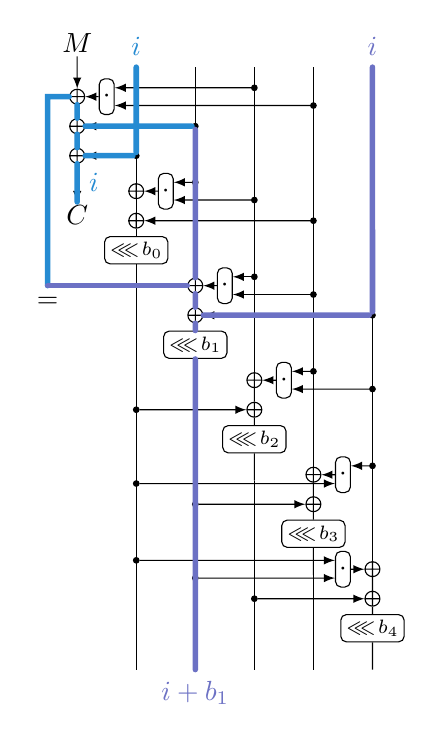
\begin{tikzpicture}[xscale=0.75,yscale=1.5]%{{{
    \printstate
    \draw[trail, beta]
      (C) -- node[right] {$i$} (lll-1)
      (lll-1) -- (tlll-1) (lll-1) -- (xor-1) (xor-1) -- (xnd-1)
      (tlll-1) -- (W-20) node[above] {$i$}
      (xor-1) -- (txor-1) %(txor-1) -- (W-21) node[above] {$i$}
      %(xnd-1) -- (and-1)
      (W40) node[below] {\phantom{$i$}}
      ;
    \draw[trail, gamma]
      %(W-21) node[above] {$i$}
      (txor-1) -- (xnd1)
      (xnd1) -- (xor1) (xor1) -- (lll1)
      %(xnd1) -- (and1)
      (xor1) -- (txor1)
      (txor1) -- (W-24) node[above] {$i$}
      (lll1) -- (W41) node[below] {$i+b_1$}
      ;
    %\draw[trail, beta,  dotted] (and-1) -- (and-1-|and1);
    %\draw[trail, gamma, dotted] (and1)  -- (and-1-|and1) node[above, black] {=};
    \draw[trail, beta]  (xnd-1) -- ++(-.5,0) coordinate (tmp) -- (tmp|-xnd1);
    \draw[trail, gamma] (tmp|-xnd1) node[below, black] {=} -- (xnd1);
  \end{tikzpicture}%}}}
  \caption*{\cipher{MiniMORUS}: weight 0 (not 2)} %$S^{j,1}_i, S^{j,4}_i, S^{j+1,1}_{i-1}$ ($w\!=\!1$)}
  \end{subfigure}
  \qquad
  \begin{subfigure}{.32\textwidth}
  \centering
  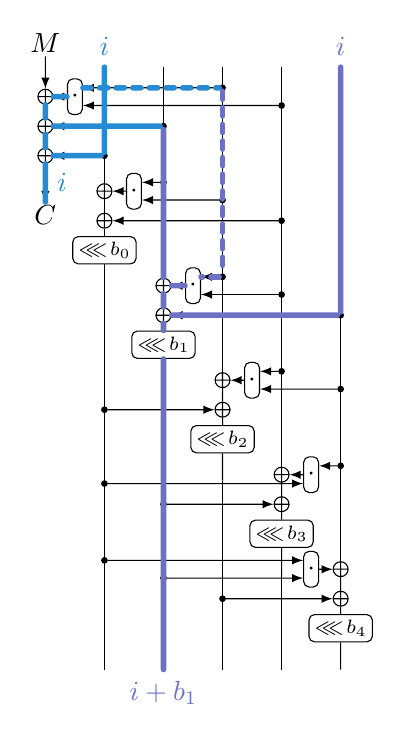
\begin{tikzpicture}[xscale=0.75,yscale=1.5]%{{{
    \printstate
    \draw[trail, beta]
      (C) -- node[right] {$i$} (lll-1)
      (lll-1) -- (tlll-1) (lll-1) -- (xor-1) (xor-1) -- (xnd-1)
      (tlll-1) -- (W-20) node[above] {$i$}
      (xor-1) -- (txor-1) %(txor-1) -- (W-21) node[above] {$i$}
      (xnd-1) -- (and-1)
      (W40) node[below] {\phantom{$i$}}
      ;
    \draw[trail, gamma]
      %(W-21) node[above] {$i$}
      (txor-1) -- (xnd1)
      (xnd1) -- (xor1) (xor1) -- (lll1)
      (xnd1) -- (and1)
      (xor1) -- (txor1)
      (txor1) -- (W-24) node[above] {$i$}
      (lll1) -- (W41) node[below] {$i+b_1$}
      ;
    \draw[trail, beta,  dashed] (and-1.east|-tanB-1) -- (tanB-1);
    \draw[trail, gamma, dashed] (tanB-1)  -- (tanB1) -- (tanB1-|and1.east);
  \end{tikzpicture}%}}}
  \caption*{\cipher{MORUS}: weight $4 \times 1$ (not $4 \times 2$)} %$S^{j,1}_i, S^{j,4}_i, S^{j+1,1}_{i-1}$ ($w\!=\!1$)}
  \end{subfigure}
  \caption{Weight of $\beta_i \oplus \gamma_i$ for \cipher{MiniMORUS} and \cipher{MORUS}.}
  \label{fig:minimorusfragments}
\end{figure}

%TODO: check $\alpha_i \oplus \beta_i \oplus \gamma_i$ in step 2 of $\cipher{MORUS-640}$
%(maybe not relevant due to overall complexity\dots)

\begin{figure}
  \newcommand{\M}[2]{1.65,-1.5*#1-.25-.25*#2}
  \newcommand{\C}[1]{-.1,-.25-1.5*#1}
  \renewcommand{\S}[2]{.25+.25*#2,-1.5*#1}
  \centering
  \begin{tikzpicture}[xscale=3, yscale=1.5, every node/.style={font=\scriptsize,inner sep=2pt}]
    \begin{scope}
      \foreach \r in {0,...,3} { \draw[gray, rounded corners=2pt] (0,-\r*1.5) rectangle ++(1.5,-1.5); }
      \foreach \r in {0,...,4} { \draw (\S{0}{\r}) node[above] {$S^{\r}$}; }
      \draw (\C{0}|-\S{0}{0}) node[above] {$C$};

      \draw[alpha] (\C{0}) node[left] {27} -| (\S{1}{0}) node[above right] {0}
                   (\M{0}{0}) node[right] {$\alpha_{27}$};

      \draw[beta]  (\C{1}) node[above left] {0} -| (\S{1}{0}) node[below right] {0}
                   (\C{1}-|\S{1}{0}) -| ([xshift=-1pt]\S{1}{1}) node[above] {0\,}
                   (\M{1}{0}) node[right] {$\beta_0$};
      \draw[alpha] ([yshift=-1.5pt]\C{1}) node[left] {8} -| (\S{2}{0}) node[above right] {\!\!13}
                   (\M{1}{1}) node[right] {$\alpha_{8,26}$};
      \draw[alpha] ([yshift=-3.0pt]\C{1}) node[below left] {26} -| ([xshift=-1pt]\S{2}{0}) node[above left] {31\!};
      \draw[gamma] (\S{1}{1}) node[above] {\,0} -- (\S{2}{1}) node[above left] {31\!\!}
                   (\S{1}{1}) ++(0,-.75) -| ([xshift=-1pt]\S{1}{4}) node[above] {0\,}
                   (\M{1}{2}) node[right] {$\gamma_0$};
      \draw[delta] (\S{1}{4}) node[above] {\,0} -- (\S{2}{4}) node[above right] {13}
                   (\S{1}{4}) ++(0,-1.25) -| ([xshift=2pt]\S{2}{2}) node[below] {0} node[black] {$\times$}
                   (\M{1}{3}) node[right] {$\delta_0$};

      \draw[beta]  (\C{2}) node[above left] {31} -| ([xshift=-1pt]\S{2}{0}) node[below left] {31\!}
                   ([xshift=-1pt]\C{2}-|\S{2}{0}) -| (\S{2}{1}) node[below left] {31\!\!}
                   (\M{2}{0}) node[right] {$\beta_{13,31}$};
      \draw[beta]  ([yshift=-1.5pt]\C{2}) node[left] {13} -| (\S{2}{0}) node[below right] {\!\!13}
                   ([yshift=-1.5pt]\C{2}-|\S{2}{0}) -| ([xshift=1pt]\S{2}{1}) node[above] {\,\,\,13};
      \draw[alpha] ([yshift=-3.0pt]\C{2}) node[below left] {7} -| (\S{3}{0}) node[above right] {12}
                   (\M{2}{1}) node[right] {$\alpha_7$};
      \draw[gamma] ([xshift=2pt]\S{2}{1}) node[below right] {13} -- ([xshift=2pt]\S{3}{1}) node[above right] {12}
                   ([xshift=2pt]\S{2}{1}) ++(0,-.75) -| (\S{2}{4}) node[below right] {13}
                   (\M{2}{2}) node[right] {$\gamma_{13}$};

      \draw[beta]  (\C{3}) node[left] {12} -| (\S{3}{0}) node[below right] {12}
                   (\C{3}-|\S{3}{0}) -| ([xshift=2pt]\S{3}{1}) node[below right] {12}
                   (\M{3}{0}) node[right] {$\beta_{12}$};

      \draw (\S{4}{2}) node[above] {\normalsize $\chi_1$: weight 7 (not 11)};
    \end{scope}

    \begin{scope}[xshift=2.5cm]
      \foreach \r in {1,...,4} { \draw[gray, rounded corners=2pt] (0,-\r*1.5) rectangle ++(1.5,-1.5); }
      \foreach \r in {0,...,4} { \draw (\S{1}{\r}) node[above] {$S^{\r}$}; }
      \draw (\C{0}|-\S{1}{0}) node[above] {$C$};

      \draw[alpha] (\C{1}) node[left] {2} -| (\S{2}{0}) node[above right] {7}
                   (\M{1}{0}) node[right] {$\alpha_{2}$};

      \draw[beta]  (\C{2}) node[above left] {7} -| (\S{2}{0}) node[below right] {7}
                   (\C{2}-|\S{2}{0}) -| ([xshift=-1pt]\S{2}{1}) node[above] {7\,}
                   (\M{2}{0}) node[right] {$\beta_7$};
      \draw[alpha] ([yshift=-1.5pt]\C{2}) node[left] {15} -| (\S{3}{0}) node[above right] {\!20}
                   (\M{2}{1}) node[right] {$\alpha_{15,1,27}$};
      \draw[alpha] ([yshift=-3.0pt]\C{2}) node[below left] {1} -| ([xshift=-1pt]\S{3}{0}) node[above left] {6\!};
      \draw[alpha] ([yshift=-4.5pt]\C{2}) node[below] {\,\,\,\,27} -| ([xshift=-3pt]\S{3}{0}) node[below] {0\,\,};
      \draw[gamma] (\S{2}{1}) node[above] {\,7} -- (\S{3}{1}) node[above left] {6\!}
                   (\S{2}{1}) ++(0,-.75) -| ([xshift=-1pt]\S{2}{4}) node[above] {7\,}
                   (\M{2}{2}) node[right] {$\gamma_7$};
      \draw[delta] (\S{2}{4}) node[above] {\,7} -- (\S{3}{4}) node[above right] {20}
                   (\S{2}{4}) ++(0,-1.25) -| ([xshift=1pt]\S{3}{2}) node[below] {\,7}
                   (\M{2}{4}) node[right] {$\delta_7$};
      \draw[epsil] (\S{2}{2}) node[above] {0} node[black] {$\times$} -- (\S{3}{2}) node[below] {7\,}
                   (\S{2}{2}) ++(0,-1.00) -| ([xshift=-4pt]\S{3}{0}) node[above left] {0}
                   (\M{2}{3}) node[right] {$\varepsilon_0$};

      \draw[beta]  (\C{3}) node[above left] {6} -| ([xshift=-1pt]\S{3}{0}) node[below left] {6\!}
                   ([xshift=-1pt]\C{3}-|\S{3}{0}) -| (\S{3}{1}) node[below left] {6\!}
                   (\M{3}{0}) node[right] {$\beta_{20,6}$};
      \draw[beta]  ([yshift=-1.5pt]\C{3}) node[left] {20} -| (\S{3}{0}) node[below right] {\!20}
                   ([yshift=-1.5pt]\C{3}-|\S{3}{0}) -| ([xshift=1pt]\S{3}{1}) node[above] {\,\,\,\,20};
      \draw[alpha] ([yshift=-3.0pt]\C{3}) node[below left] {14} -| (\S{4}{0}) node[above right] {19}
                   (\M{3}{1}) node[right] {$\alpha_{14}$};
      \draw[gamma] ([xshift=2pt]\S{3}{1}) node[below right] {20} -- ([xshift=2pt]\S{4}{1}) node[above right] {19}
                   ([xshift=2pt]\S{3}{1}) ++(0,-.75) -| (\S{3}{4}) node[below right] {20}
                   (\M{3}{2}) node[right] {$\gamma_{20}$};

      \draw[beta]  (\C{4}) node[left] {19} -| (\S{4}{0}) node[below right] {19}
                   (\C{4}-|\S{4}{0}) -| ([xshift=2pt]\S{4}{1}) node[below right] {19}
                   (\M{4}{0}) node[right] {$\beta_{19}$};

      \draw (\S{5}{2}) node[above] {\normalsize $\chi_2$: weight 9 (not 13)};
      \draw (\S{0}{2}) node[below] {\normalsize \cipher{MiniMORUS-640}};
    \end{scope}

    \draw[dashed] (\S{4.25}{-1}) -- (\S{4.25}{7}) -- ++(\S{1}{-1}) -- ++(\S{0}{7});

    \begin{scope}[yshift=-7.0cm]
      \foreach \r in {0,...,3} { \draw[gray, rounded corners=2pt] (0,-\r*1.5) rectangle ++(1.5,-1.5); }
      \foreach \r in {0,...,4} { \draw (\S{0}{\r}) node[above] {$S^{\r}$}; }
      \draw (\C{0}|-\S{0}{0}) node[above] {$C$};

      \draw[alpha] (\C{0}) node[left] {51} -| (\S{1}{0}) node[above right] {0}
                   (\M{0}{0}) node[right] {$\alpha_{51}$};

      \draw[beta]  (\C{1}) node[above left] {0} -| (\S{1}{0}) node[below right] {0}
                   (\C{1}-|\S{1}{0}) -| ([xshift=-1pt]\S{1}{1}) node[above] {0\,}
                   (\M{1}{0}) node[right] {$\beta_0$};
      \draw[alpha] ([yshift=-1.5pt]\C{1}) node[left] {55} -| (\S{2}{0}) node[above right] {\!4}
                   (\M{1}{1}) node[right] {$\alpha_{55,33}$};
      \draw[alpha] ([yshift=-3.0pt]\C{1}) node[below left] {33} -| ([xshift=-1pt]\S{2}{0}) node[above left] {46\!};
      \draw[gamma] (\S{1}{1}) node[above] {\,0} -- (\S{2}{1}) node[above left] {46\!}
                   (\S{1}{1}) ++(0,-.75) -| ([xshift=-1pt]\S{1}{4}) node[above] {0\,}
                   (\M{1}{2}) node[right] {$\gamma_0$};
      \draw[delta] (\S{1}{4}) node[above] {\,0} -- (\S{2}{4}) node[above right] {4}
                   (\S{1}{4}) ++(0,-1.25) -| ([xshift=2pt]\S{2}{2}) node[below] {0} node[black] {$\times$}
                   (\M{1}{3}) node[right] {$\delta_0$};

      \draw[beta]  (\C{2}) node[above left] {46} -| ([xshift=-1pt]\S{2}{0}) node[below left] {46\!}
                   ([xshift=-1pt]\C{2}-|\S{2}{0}) -| (\S{2}{1}) node[below left] {46\!}
                   (\M{2}{0}) node[right] {$\beta_{4,46}$};
      \draw[beta]  ([yshift=-1.5pt]\C{2}) node[left] {4} -| (\S{2}{0}) node[below right] {\!4}
                   ([yshift=-1.5pt]\C{2}-|\S{2}{0}) -| ([xshift=1pt]\S{2}{1}) node[above] {\,\,\,4};
      \draw[alpha] ([yshift=-3.0pt]\C{2}) node[below left] {37} -| (\S{3}{0}) node[above right] {50}
                   (\M{2}{1}) node[right] {$\alpha_{37}$};
      \draw[gamma] ([xshift=2pt]\S{2}{1}) node[below right] {4} -- ([xshift=2pt]\S{3}{1}) node[above right] {50}
                   ([xshift=2pt]\S{2}{1}) ++(0,-.75) -| (\S{2}{4}) node[below right] {4}
                   (\M{2}{2}) node[right] {$\gamma_{4}$};

      \draw[beta]  (\C{3}) node[left] {50} -| (\S{3}{0}) node[below right] {50}
                   (\C{3}-|\S{3}{0}) -| ([xshift=2pt]\S{3}{1}) node[below right] {50}
                   (\M{3}{0}) node[right] {$\beta_{50}$};

      \draw (\S{4}{2}) node[above] {\normalsize $\chi_1$: weight 7 (not 11)};
      \draw (\S{5}{2}) node[above] {\normalsize \cipher{MiniMORUS-1280}};
    \end{scope}

    \begin{scope}[xshift=2.5cm,yshift=-7.0cm]
      \foreach \r in {1,...,4} { \draw[gray, rounded corners=2pt] (0,-\r*1.5) rectangle ++(1.5,-1.5); }
      \foreach \r in {0,...,4} { \draw (\S{1}{\r}) node[above] {$S^{\r}$}; }
      \draw (\C{0}|-\S{1}{0}) node[above] {$C$};

      \draw[alpha] (\C{1}) node[left] {25} -| (\S{2}{0}) node[above right] {38}
                   (\M{1}{0}) node[right] {$\alpha_{25}$};

      \draw[beta]  (\C{2}) node[above left] {38} -| (\S{2}{0}) node[below right] {38}
                   (\C{2}-|\S{2}{0}) -| ([xshift=-1pt]\S{2}{1}) node[above] {38\,}
                   (\M{2}{0}) node[right] {$\beta_{38}$};
      \draw[alpha] ([yshift=-1.5pt]\C{2}) node[left] {7} -| (\S{3}{0}) node[above right] {\!20}
                   (\M{2}{1}) node[right] {$\alpha_{7,1,51}$};
      \draw[alpha] ([yshift=-3.0pt]\C{2}) node[below left] {29} -| ([xshift=-1pt]\S{3}{0}) node[above left] {42\!};
      \draw[alpha] ([yshift=-4.5pt]\C{2}) node[below] {\,\,\,\,51} -| ([xshift=-4pt]\S{3}{0}) node[below] {0\,\,\,};
      \draw[gamma] (\S{2}{1}) node[above right] {38} -- (\S{3}{1}) node[above left] {20\!}
                   (\S{2}{1}) ++(0,-.75) -| ([xshift=-1pt]\S{2}{4}) node[above left] {38}
                   (\M{2}{2}) node[right] {$\gamma_{38}$};
      \draw[delta] (\S{2}{4}) node[above] {\,38} -- (\S{3}{4}) node[above right] {42}
                   (\S{2}{4}) ++(0,-1.25) -| ([xshift=1pt]\S{3}{2}) node[below right] {38}
                   (\M{2}{4}) node[right] {$\delta_{38}$};
      \draw[epsil] (\S{2}{2}) node[above] {0} node[black] {$\times$} -- (\S{3}{2}) node[below] {38}
                   (\S{2}{2}) ++(0,-1.00) -| ([xshift=-5pt]\S{3}{0}) node[above left] {0}
                   (\M{2}{3}) node[right] {$\varepsilon_0$};

      \draw[beta]  (\C{3}) node[above left] {42} -| ([xshift=-1pt]\S{3}{0}) node[below left] {42\!}
                   ([xshift=-1pt]\C{3}-|\S{3}{0}) -| (\S{3}{1}) node[below left] {42\!}
                   (\M{3}{0}) node[right] {$\beta_{20,42}$};
      \draw[beta]  ([yshift=-1.5pt]\C{3}) node[left] {20} -| (\S{3}{0}) node[below right] {\!20}
                   ([yshift=-1.5pt]\C{3}-|\S{3}{0}) -| ([xshift=1pt]\S{3}{1}) node[above] {\,\,\,\,20};
      \draw[alpha] ([yshift=-3.0pt]\C{3}) node[below left] {11} -| (\S{4}{0}) node[above right] {24}
                   (\M{3}{1}) node[right] {$\alpha_{11}$};
      \draw[gamma] ([xshift=2pt]\S{3}{1}) node[below right] {42} -- ([xshift=2pt]\S{4}{1}) node[above right] {24}
                   ([xshift=2pt]\S{3}{1}) ++(0,-.75) -| (\S{3}{4}) node[below right] {42}
                   (\M{3}{2}) node[right] {$\gamma_{42}$};

      \draw[beta]  (\C{4}) node[left] {24} -| (\S{4}{0}) node[below right] {24}
                   (\C{4}-|\S{4}{0}) -| ([xshift=2pt]\S{4}{1}) node[below right] {24}
                   (\M{4}{0}) node[right] {$\beta_{24}$};

      \draw (\S{5}{2}) node[above] {\normalsize $\chi_2$: weight 9 (not 13)};
    \end{scope}
  \end{tikzpicture}
  \caption{\cipher{MiniMORUS}: Two approximations for $S^{2,2}_0$}
\end{figure}

\clearpage

\section{Linear Approximations for \cipher{MORUS}}

\section{Differential Attack on the Finalization}

\section{Key-Recovery Attack in Nonce-Misuse Setting}

\end{document}
